\begin{ExerciseList}

  \setcounter{Exercise}{0}
  \section{Lab 3: User Environments}

  \subsection{实验目的}

  在这个实验中,我们将实现操作系统的一些基本功能,来实现用户环境下的进程的正常运行。你将会加强JOS内核的功能,为它增添一些重要的数据结构,用来记录用户进程环境的一些信息;创建一个单一的用户环境,并且加载一个程序运行它。你也可以让JOS内核能够完成用户环境所作出的任何系统调用,以及处理用户环境产生的各种异常。

  \subsection{实验内容}

这个实验 多了很多代码

\begin{itemize}
\item INC/env.h	用户模式环境的公共定义
\item trap.h	陷阱处理的公共定义
\item syscall.h	从用户环境到内核的系统调用的公共定义
\item lib.h	用户模式支持库的公共定义
\item kern/env.h	用户模式环境的内核专用定义
\item env.c	内核代码实现用户模式环境
\item trap.h	内核专用陷阱处理定义
\item trap.c	陷阱处理代码
\item trapentry.S	汇编语言陷阱处理程序入口点
\item syscall.h	系统调用处理的内核专用定义
\item syscall.c	系统调用实现代码
\item Lib/Makefrag	Makefile片段构建用户模式库 obj / lib / libjos.a
\item entry.S中	用户环境的汇编语言入口
\item libmain.c	来自entry.S的用户模式库设置代码
\item syscall.c	用户模式系统调用存根函数
\item console.c中	putchar和getchar的用户模式实现,控制台I / O
\item exit.c中	用户模式执行的退出
\item panic.c	用户模式执行 panic
\item user/\*	各种测试程序来检查内核实验3代码
\end{itemize}

操作系统维护了三个重要的全局变量

\begin{minted}{C}
  struct Env *envs = NULL;//所有的 Env 结构体
  struct Env *curenv = NULL; //目前正在运行的用户环境
  static struct Env *env_free_list;
  //还没有被使用的 Env 结构体链表
\end{minted}

内核刚启动的时候,curenv的值为NULL。

具体Env 结构体定义:

  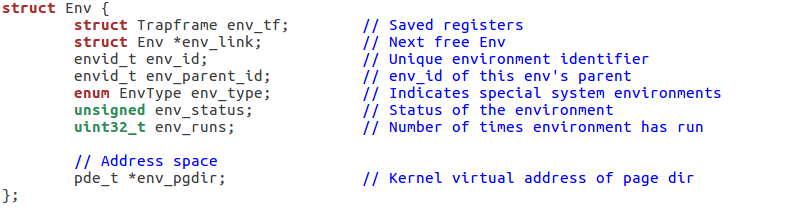
\includegraphics[width=6in]{figures/lab2/image52.png}


\begin{itemize}
  \item env\_tf:\\
      这个类型的结构体在inc/trap.h文件中被定义,里面存放着当用户环境暂停运行时,所有重要寄存器的值。内核也会在系统从用户态切换到内核态时保存这些值,这样的话用户环境可以在之后被恢复,继续执行。
  \item env\_link:\\
      这个指针指向在env\_free\_list中,该结构体的后一个free的Env结构体。当然前提是这个结构体还没有被分配给任意一个用户环境时,该域才有用。
  \item env\_id:\\
      这个值可以唯一的确定使用这个结构体的用户环境是什么。当这个用户环境终止,内核会把这个结构体分配给另外一个不同的环境,这个新的环境会有不同的env\_id值。
  \item env\_parent\_id:\\
    创建这个用户环境的父用户环境的env\_id
  \item env\_type:\\
    用于区别出来某个特定的用户环境。对于大多数环境来说,它的值都是 ENV\_TYPE\_USER.
  \item env\_status:\\
    这个变量存放以下可能的值
  \item ENV\_FREE:\\
    代表这个结构体是不活跃的,应该在链表env\_free\_list中。
  \item ENV\_RUNNABLE: \\
    代表这个结构体对应的用户环境已经就绪,等待被分配处理机。
  \item ENV\_RUNNING:\\
    代表这个结构体对应的用户环境正在运行。
  \item ENV\_NOT\_RUNNABLE: \\
    代表这个结构体所代表的是一个活跃的用户环境,但是它不能被调度运行,因为它在等待其他环境传递给它的消息。
  \item ENV\_DYING: \\
    代表这个结构体对应的是一个僵尸环境。一个僵尸环境在下一次陷入内核时会被释放回收。
  \item env\_pgdir:\\
    这个变量存放着这个环境的页目录的虚拟地址
\end{itemize}

\Exercise{现在你需要进一步去修改mem\_init()函数,来分配一个Env结构体数组,叫做envs。}

这个实验在做了lab2的实验之后就很好做了。

  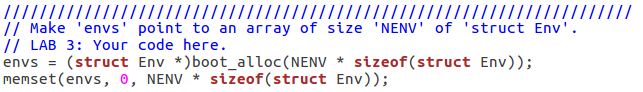
\includegraphics[width=6in]{figures/lab2/image53.png}

我们现在需要来运行一个用户环境,我们需要把内核设置成能够加载内核中的静态二进制文件。


\Exercise{region\_alloc(): 为用户环境分配物理地址空间}

   load\_icode(): 分析一个ELF文件,类似于boot loader做的那样,我们可以把它的内容加载到用户环境下。

   env\_create(): 利用env\_alloc函数和load\_icode函数,加载一个ELF文件到用户环境中

   env\_run(): 在用户模式下,开始运行一个用户环境。

  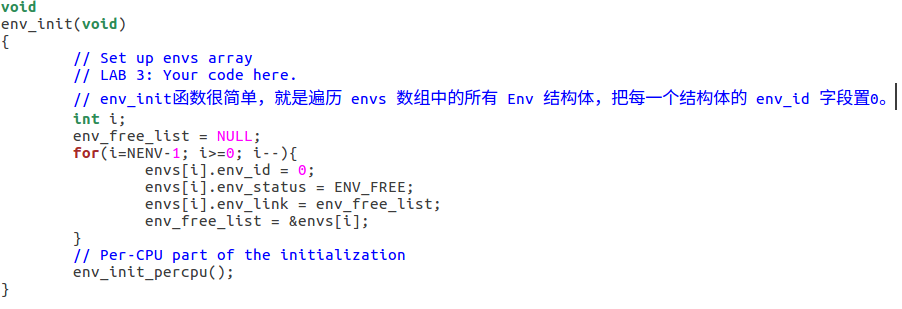
\includegraphics[width=6in]{figures/lab2/image54.png}

这是env\_init():初始化所有的在envs数组中的 Env结构体,并把它们加入到 env\_free\_list中。 还要调用 env\_init\_percpu,这个函数要配置段式内存管理系统,让它所管理的段,可能具有两种访问优先级其中的一种,一个是内核运行时的0优先级,以及用户运行时的3优先级。

 env\_setup\_vm(): 为一个新的用户环境分配一个页目录表,并且初始化这个用户环境的地址空间中的和内核相关的部分。

  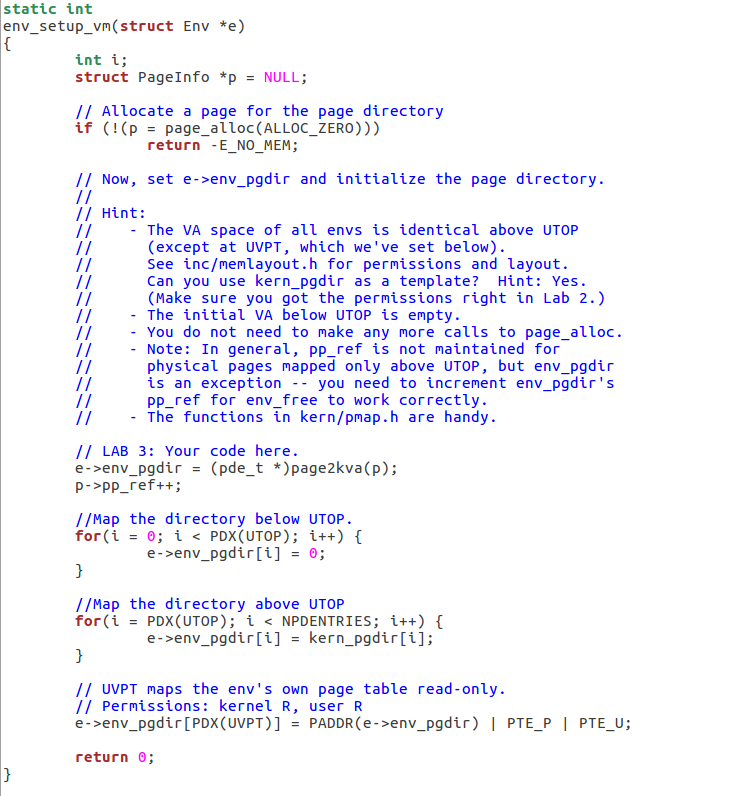
\includegraphics[width=6in]{figures/lab2/image55.png}

  region\_alloc 为用户环境分配物理空间,这里注意我们要先把起始地址和终止地址进行页对齐,对其之后我们就可以以页为单位,为其一个页一个页的分配内存,并且修改页目录表和页表。

  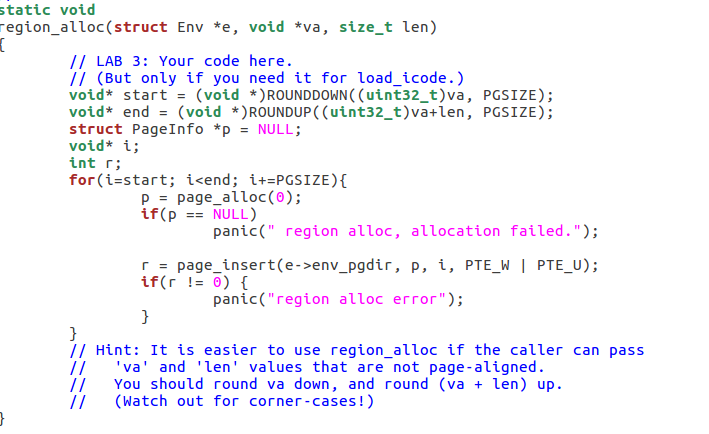
\includegraphics[width=6in]{figures/lab2/image56.png}

  load\_icode 功能是为每一个用户进程设置它的初始代码区,堆栈以及处理器标识位。每个用户程序都是ELF文件,所以我们要解析该ELF文件。

  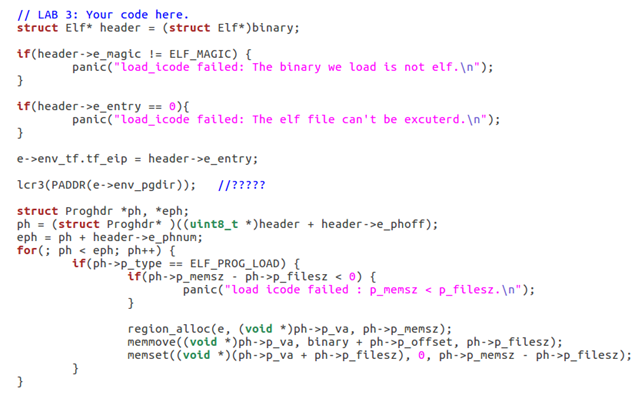
\includegraphics[width=6in]{figures/lab2/image57.png}

  env\_create 是利用env\_alloc函数和load\_icode函数,加载一个ELF文件到用户环境中。

  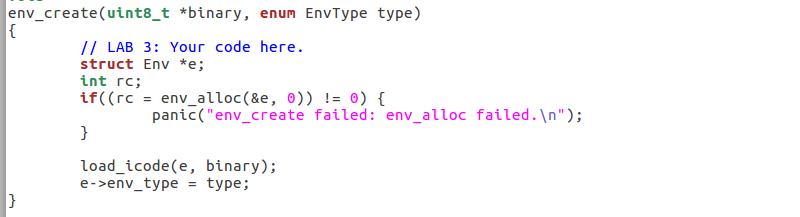
\includegraphics[width=6in]{figures/lab2/image58.png}

  env\_run 是真正开始运行一个用户环境

  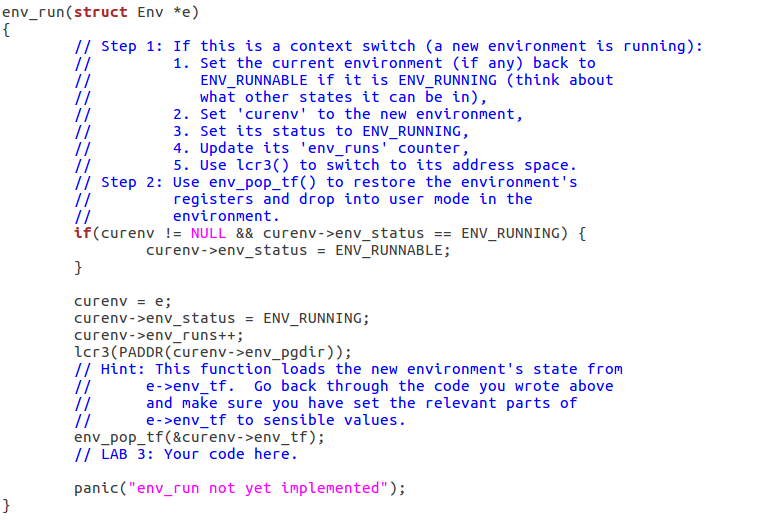
\includegraphics[width=6in]{figures/lab2/image59.png}

  用户环境的代码被调用前,操作系统一共按顺序执行了以下几个函数:

  * start (kern/entry.S)

  * i386\_init (kern/init.c)

  cons\_init

  mem\_init

  env\_init

  trap\_init (目前还未实现)

  env\_create

  env\_run

  env\_pop\_tf

显然用户级线程是不可以调用系统内存的,因为现在系统无法从用户态切换到内核态。所以你需要实现一个基本的异常/系统调用处理机制,使得内核可以从用户态转换为内核态。

\begin{enumerate}
\item 中断向量表:\\
     处理器保证中断和异常只能够引起内核进入到一些特定的,被事先定义好的程序入口点,而不是由触发中断的程序来决定中断程序入口点。\\
     X86允许多达256个不同的中断和异常,每一个都配备一个独一无二的中断向量。一个向量指的就是0到255中的一个数。一个中断向量的值是根据中断源来决定的:不同设备,错误条件,以及对内核的请求都会产生出不同的中断和中断向量的组合。CPU将使用这个向量作为这个中断在中断向量表中的索引,这个表是由内核设置的,放在内核空间中,和GDT很像。通过这个表中的任意一个表项,处理器可以知道:\\
   *需要加载到EIP寄存器中的值,这个值指向了处理这个中断的中断处理程序的位置。\\
   *需要加载到CS寄存器中的值,里面还包含了这个中断处理程序的运行特权级。(即这个程序是在用户态还是内核态下运行。)\\
\item 任务状态段\\
   处理器还需要一个地方来存放,当异常/中断发生时,处理器的状态,比如EIP和CS寄存器的值。这样的话,中断处理程序一会可以重新返回到原来的程序中。这段内存自然也要保护起来,不能被用户态的程序所篡改。\\
   正因为如此,当一个x86处理器要处理一个中断,异常并且使运行特权级从用户态转为内核态时,它也会把它的堆栈切换到内核空间中。一个叫做 “任务状态段(TSS)”的数据结构将会详细记录这个堆栈所在的段的段描述符和地址。处理器会把SS,ESP,EFLAGS,CS,EIP以及一个可选错误码等等这些值压入到这个堆栈上。然后加载中断处理程序的CS,EIP值,并且设置ESP,SS寄存器指向新的堆栈。\\
    尽管TSS非常大,并且还有很多其他的功能,但是JOS仅仅使用它来定义处理器从用户态转向内核态所采用的内核堆栈,由于JOS中的内核态指的就是特权级0,所以处理器用TSS中的ESP0,SS0字段来指明这个内核堆栈的位置,大小。
\end{enumerate}

\textbf{扩展0-31号中断}

\begin{enumerate}
\item trap\_init() 先将所有中断处理函数的起始地址放到中断向量表IDT中。

   \item 当中断发生时,不管是外部中断还是内部中断,处理器捕捉到该中断,进入核心态,根据中断向量去查询中断向量表,找到对应的表项
  \item 保存被中断的程序的上下文到内核堆栈中,调用这个表项中指明的中断处理函数。
  \item 执行中断处理函数。
\item 执行完成后,恢复被中断的进程的上下文,返回用户态,继续运行这个进程。
\item	阅读 第9章异常和中断 的 80386程序员手册 (或第5章 IA-32开发者手册)
\end{enumerate}

\Exercise{编辑一下trapentry.S 和 trap.c 文件,并且实现上面所说的功能。宏定义 TRAPHANDLER 和 TRAPHANDLER\_NOEC 会对你有帮助。你将会在 trapentry.S文件中为在inc/trap.h文件中的每一个trap加入一个入口指, 你也将会提供\_alttraps的值。}

需要修改trap\_init()函数来初始化idt表,使表中每一项指向定义在trapentry.S中的入口指针,SETGATE宏定义在这里用得上。

你所实现的 \_alltraps 应该:

\begin{enumerate}
\item 把值压入堆栈使堆栈看起来像一个结构体 Trapframe
\item 加载 GD\_KD 的值到 %ds, %es寄存器中
\item 把\%esp的值压入,并且传递一个指向Trapframe的指针到trap()函数中。
\item 调用trap trapentry.S
\end{enumerate}

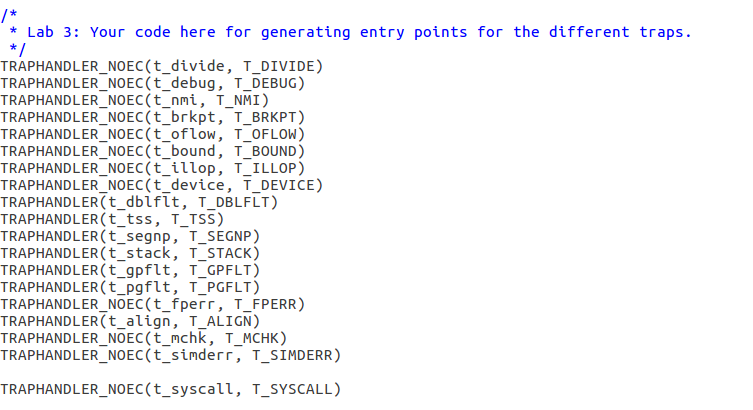
\includegraphics[width=6in]{figures/lab2/image62.png}

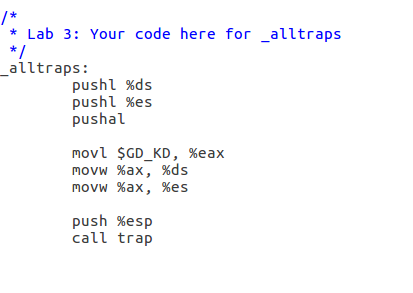
\includegraphics[width=6in]{figures/lab2/image61.png}

对于trap\_init定义如下:

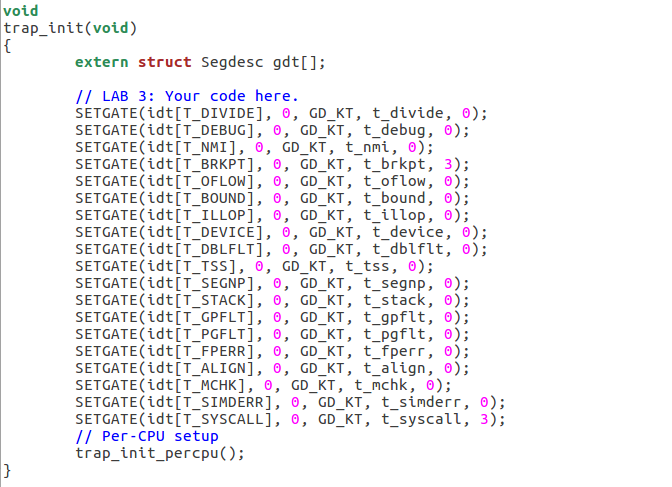
\includegraphics[width=6in]{figures/lab2/image63.png}

  \Exercise{这个练习和上一个基本类似}

  断点异常,异常号为3,这个异常可以让调试器能够给程序加上断点。加断点的基本原理就是把要加断点的语句用一个 INT3 指令替换,执行到INT3时,会触发软中断。在JOS中,我们将通过把这个异常转换成一个伪系统调用,这样的话任何用户环境都可以使用这个伪系统调用来触发JOS kernel monitor。

  问答:在上面的break point exception测试程序中,如果你在设置IDT时,对break point exception采用不同的方式进行设置,可能会产生触发不同的异常,有可能是break point exception,有可能是 general protection exception。这是为什么?你应该怎么做才能得到一个我们想要的breakpoint exception,而不是general protection exception?

  答:通过实验发现出现这个现象的问题就是在设置IDT表中的breakpoint exception的表项时,如果我们把表项中的DPL字段设置为3,则会触发break point exception,如果设置为0,则会触发general protection exception。DPL字段代表的含义是段描述符优先级(Descriptor Privileged Level),如果我们想要当前执行的程序能够跳转到这个描述符所指向的程序哪里继续执行的话,有个要求,就是要求当前运行程序的CPL,RPL的最大值需要小于等于DPL,否则就会出现优先级低的代码试图去访问优先级高的代码的情况,就会触发general protection exception。那么我们的测试程序首先运行于用户态,它的CPL为3,当异常发生时,它希望去执行 int 3指令,这是一个系统级别的指令,用户态命令的CPL一定大于 int 3 的DPL,所以就会触发general protection exception,但是如果把IDT这个表项的DPL设置为3时,就不会出现这样的现象了,这时如果再出现异常,肯定是因为我们还没有编写处理break point exception的程序所引起的,所以是break point exception。

  \Exercise{给中断向量T\_SYSCALL编写一个中断处理函数。你需要去编辑kern/trapentry.S和kern/trap.c中的trap\_init()函数。你也需要去修改trap\_dispatch()函数,使他能够通过调用syscall()(在kern/syscall.c中定义的)函数处理系统调用中断。最终你需要去实现kern/syscall.c中的syscall()函数。确保这个函数会在系统调用号为非法值时返回-E\_INVAL。你应该充分理解lib/syscall.c文件。我们要处理在inc/syscall.h文件中定义的所有系统调用。}

  我们需要了解一下系统调用的整个流程,如果现在运行的是内核态的程序的话,此时调用了一个系统调用,比如 sys\_cputs 函数时,此时不会触发中断,那么系统会直接执行定义在 lib/syscall.c 文件中的 sys\_cputs,我们可以看一下这个文件,可以发现这个文件中定义了几个比较常用的系统调用,包括 sys\_cputs, sys\_cgetc 等等。我们还会发现他们都是统一调用一个 syscall 函数,通过这个函数的代码发现其实它是执行了一个汇编指令。所以最终是这个函数完成了系统调用。以上是运行在内核态下的程序,调用系统调用时的流程。但是如果是用户态程序呢?这个练习就是让我们编写程序使我们的用户程序在调用系统调用时,最终也能经过一系列的处理最终去执行 lib/syscall.c 中的 syscall 指令。让我们看一下这个过程,当用户程序中要调用系统调用时,比如 sys\_cputs,从它的汇编代码中我们会发现,它会执行一个 int \$0x30 指令,这个指令就是软件中断指令,这个中断的中断号就是 0x30,即 T\_SYSCALL,所以题目中让我们首先为这个中断号编写一个中断处理函数,我们首先就要在 kern/trapentry.S 文件中为它声明它的中断处理函数,即TRAPHANDLER\_NOEC,就像我们为其他中断号所做的那样。

  所以我们可以假象一下,是不是 kern/syscall.c 中的 syscall 就是一个外壳函数,它的存在就是为了能够调用 lib/syscall 的呢? 所以我们按照这个思路继续进行下去,我们再继续观察 kern/syscall.c 中的其他函数,会惊人的发现,kern/syscall.c 中的所有函数居然和 lib/syscall.c 中的所有函数都是一样的!!比如 在这两个文件中都有 sys\_cputs 函数,但是我们仔细观察可以发现这两个同名的函数,实现方式却不一样。

  其实系统调用,syscall函数需要处理各种函数的信息

  \Exercise{用户程序真正开始运行的地方是在lib/entry.S文件中。该文件中,首先会进行一些设置,然后就会调用lib/libmain.c 文件中的 libmain() 函数。你首先要修改一下 libmain() 函数,使它能够初始化全局指针 thisenv ,让它指向当前用户环境的 Env 结构体。}

  然后 libmain() 函数就会调用 umain,这个 umain 程序恰好是 user/hello.c 中被调用的函数。在之前的实验中我们发现,hello.c程序只会打印 "hello, world" 这句话,然后就会报出 page fault 异常,原因就是 thisenv->env\_id 这条语句。现在你已经正确初始化了这个 thisenv的值,再次运行就应该不会报错了。

  其实这个练习就是让你通过程序获得当前正在运行的用户环境的 env\_id , 以及这个用户环境所对应的 Env 结构体的指针。 env\_id 我们可以通过调用 sys\_getenvid() 这个函数来获得。那么如何获得它对应的 Env结构体指针呢?

  通过阅读 lib/env.h 文件我们知道,env\_id的值包含三部分,第31位被固定为0;第10~30这21位是标识符,标示这个用户环境;第0~9位代表这个用户环境所采用的 Env 结构体,在envs数组中的索引。所以我们只需知道 env\_id 的低 0~9 位,我们就可以获得这个用户环境对应的 Env 结构体了。

\Exercise{内存保护是操作系统的非常重要的一项功能,它可以防止由于用户程序崩溃对操作系统带来的破坏与影响。操作系统通常依赖于硬件的支持来实现内存保护。操作系统可以让硬件能够始终知晓哪些虚拟地址是有效的,哪些是无效的。当程序尝试去访问一个无效地址,或者尝试去访问一个超出它访问权限的地址时,处理器会在这个指令处终止,并且触发异常,陷入内核态,与此同时把错误的信息报告给内核。如果这个异常是可以被修复的,那么内核会修复这个异常,然后程序继续运行。如果异常无法被修复,则程序永远不会继续运行。}

 作为一个可修复异常的例子,让我们考虑一下可自动扩展的堆栈。在许多系统中,内核在初始情况下只会分配一个内核堆栈页,如果程序想要访问这个内核堆栈页之外的堆栈空间的话,就会触发异常,此时内核会自动再分配一些页给这个程序,程序就可以继续运行了。

 系统调用也为内存保护带来了问题。大部分系统调用接口让用户程序传递一个指针参数给内核。这些指针指向的是用户缓冲区。通过这种方式,系统调用在执行时就可以解引用这些指针。但是这里有两个问题:

 1. 在内核中的page fault要比在用户程序中的page fault更严重。如果内核在操作自己的数据结构时出现 page faults,这是一个内核的bug,而且异常处理程序会中断整个内核。但是当内核在解引用由用户程序传递来的指针时,它需要一种方法去记录此时出现的任何page faults都是由用户程序带来的。

 2. 内核通常比用户程序有着更高的内存访问权限。用户程序很有可能要传递一个指针给系统调用,这个指针指向的内存区域是内核可以进行读写的,但是用户程序不能。此时内核必须小心不要去解析这个指针,否则的话内核的重要信息很有可能被泄露。

  现在你需要通过仔细检查所有由用户传递来指针所指向的空间来解决上述两个问题。当一个程序传递给内核一个指针时,内核会检查这个地址是在整个地址空间的用户地址空间部分,而且页表也运行进行内存的操作。

修改kern/trap.c文件,使其能够实现:当在内核模式下发现页错,trap.c 文件会panic。

提示:

为了能够判断这个page fault是出现在内核模式下还是用户模式下,我们应该检查 tf\_cs 的低几位。

阅读 user\_mem\_assert (在 kern/pmap.c),并且实现 user\_mem\_check;

修改一下 kern/syscall.c 去检查输入参数。

启动内核后,运行 user/buggyhello 程序,用户环境可以被销毁,内核不可以panic,你应该看到:

[00001000] user\_mem\_check assertion failure for va 00000001

[00001000] free env 00001000

Destroyed the only environment - nothing more to do!

首先我们应该根据什么来判断当前运行的程序时处在内核态下还是用户态下?答案是根据 CS 段寄存器的低2位,这两位的名称叫做 CPL 位,表示当前运行的代码的访问权限级别,0代表是内核态,3代表是用户态。

题目要求我们在检测到这个 page fault 是出现在内核态时,要把这个事件 panic 出来,所以我们把 page\_fault\_handler 文件修改如下:

user\_mem\_check 函数的功能是检查一下当前用户态程序是否有对虚拟地址空间 [va, va+len] 的 perm| PTE\_P 访问权限。自然我们要做的事情应该是,先找到这个虚拟地址范围对应于当前用户态程序的页表中的页表项,然后再去看一下这个页表项中有关访问权限的字段,是否包含 perm | PTE\_P,只要有一个页表项是不包含的,就代表程序对这个范围的虚拟地址没有 perm|PTE\_P 的访问权限。以上就是这段代码的大致思想。

其中syscall中的sys\_cputs函数,这个函数对虚拟地址检查权限。

运行后可以看到

\Exercise{没有新东西,就是测试练习9的代码}

\end{ExerciseList}
